\documentclass[11pt]{beamer}
\usetheme{Warsaw}
\usepackage[czech]{babel}
\usepackage[utf8]{inputenc}
\usepackage{amsmath}
\usepackage{amsfonts}
\usepackage{amssymb}
\usepackage{graphicx}
\author{Vojtěch Krákora \\ Tomáš Šabata}
%\title{Aplikace pro vyhodnocení stylu jízdy řidiče}
\title[\hspace{50mm} \insertframenumber/\inserttotalframenumber]{Normalized cuts}
\institute{České vysoké učení technické v Praze} 
\date{} 
%\subject{} 
\begin{document}

\begin{frame}
\titlepage
\end{frame}

\begin{frame}
\tableofcontents
\end{frame}

\section{Princip}
\begin{frame}
\begin{itemize}
\item $G=(V,E), V \rightarrow$ pixely, $E \rightarrow$ míra podobnosti mezi uzly.
\item Míra podobnosti $w(x,y)=e^{-\frac{||color(x) - color(y)||}{\sigma}} * e^{-\frac{||distance(x,y)||}{\sigma}}$
\item Hledání normalizovaného minimálního řezu grafu.

\begin{center}
\item
$Ncut(a,b)=\frac{cut(A,B)}{assoc(A,V)}+\frac{cut(A,B)}{assoc(B,V)}$

$ assoc(A,V)=\sum_{u\in A, t\in V} w(u,t)$

\end{center}
\item To je NP-Úplný problém $\rightarrow$ aproximace
\end{itemize}
\end{frame}

\begin{frame}
\begin{itemize}
\item $min_xNcut(x)=min_y\frac{y^T(D-A)y}{y^TDy}, y(i)\in\{1,-b\},y^TD1=0$
\item Převede se na řešení rovnice $(D-A)y=\lambda Dy$
\item Zjednodušení na $D^{-\frac{1}{2}}(D-A)D^{-\frac{1}{2}}v=\lambda v$
\item $D=|G(V)|$ x $|G(V)|$ matice stupně (degree matrix)
\item $A=|G(V)|$ x $|G(V)|$ matice podobnosti (affinity matrix)
\item $D_{i,i}=\sum_{j\in V}d(i,j)$,$D_{i,j;i\neq j}=0$
\item $A_{i,j}=d(i,j)$
\end{itemize}
\end{frame}
\section{Algoritmus}
\begin{frame}
\begin{enumerate}
\item Reprezentace obrázku jako grafu G = (V,E).
\item Vytvoření matice A a D.
\item Výpočet vlastního vektoru druhého nejmenšího vlastního čísla.
\item Rozdělení grafu G na dvě disjunktní množiny A, B pomocí vlastního vektoru.
\item Rekurzivně opakovat na množinách A, B v případě nestabilního řezu.
\end{enumerate}

\end{frame}
\section{Výsledky segmentace}
\begin{frame}
\begin{center}
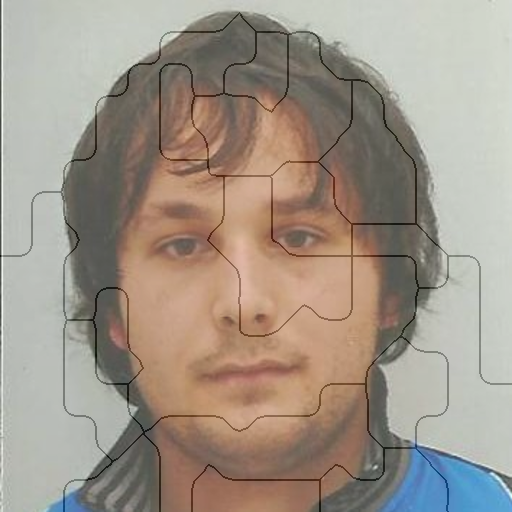
\includegraphics[scale=0.40]{images/emb1_1_1.png}
\end{center}
\end{frame}

\begin{frame}
\begin{center}
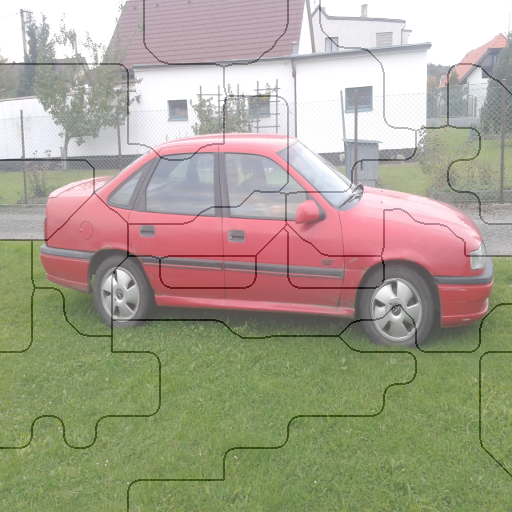
\includegraphics[scale=0.40]{images/emb1_1_2.png}
\end{center}
\end{frame}


\begin{frame}
\begin{center}
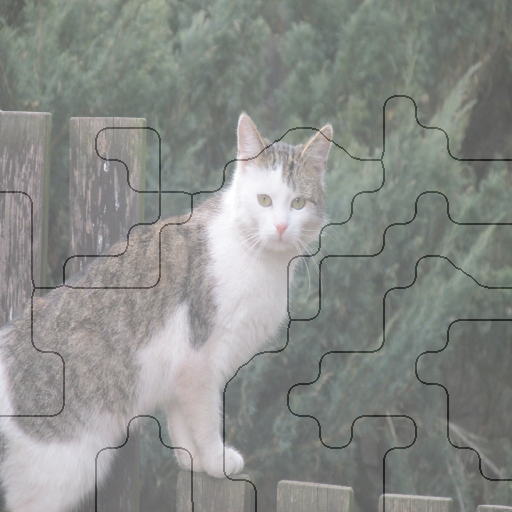
\includegraphics[scale=0.40]{images/emb1_2_1.png}
\end{center}
\end{frame}


\begin{frame}
\begin{center}
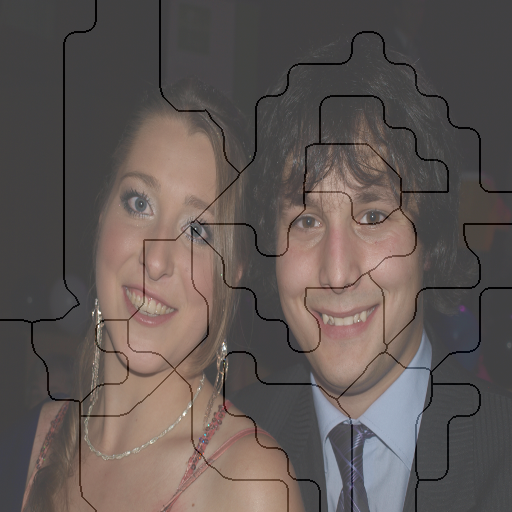
\includegraphics[scale=0.40]{images/emb1_2_2.png}
\end{center}
\end{frame}


\section*{Zdroje}
\begin{frame}
\begin{thebibliography}{9}
\bibitem{shi}
SHI, Jianbo a J. MALIK. Normalized cuts and image segmentation. \textit{IEEE Transactions on Pattern Analysis and Machine Intelligence} [online]. 2000, vol.~22, issue 8, s.~888-905 [cit. 2014-12-13]. DOI: 10.1109/34.868688. 
\end{thebibliography}
\end{frame}


\end{document}